%======================================================================
\chapter{Introduction}
%======================================================================

Quantitative risk management is a key component of modern financial systems, ensuring the stability and resilience of markets, institutions, and portfolios against an array of risks. 
For financial products like option portfolios and variable annuity (VA) contracts, traditional risk assessment methods often fall short in accurately capturing the complex dynamics of the underlying risk factors.
VA contracts are a popular type of complex insurance product that is linked to the performance of underlying assets, providing a guaranteed minimum income benefit to the policyholder.
This is where advanced Monte Carlo simulation techniques, particularly nested simulation procedures, become indispensable.
In contrast to finite-difference methods, a Monte Carlo simulation scheme is more flexible and can be easily adapted to model tail risk with a rule-based design.
~\cite{glasserman2004monte} provide a comprehensive overview of nested simulation methods in financial engineering and risk management applications.
In this thesis, we focus on building and analyzing nested simulation procedures for risk management applications of financial derivatives and insurance products.
Nested simulation, also known as nested stochastic modeling and stochastic-on-stochastic modeling, becomes necessary when stochastic simulation of a parameter of interest is contingent on another quantity to be determined stochastically.
In the context of financial engineering, nested simulation is used to model the tail risk of a contract whose payoff depends on a set of underlying risk factors.
For example, estimating the value of an exotic option at a risk horizon requires simulation given a realization of the underlying assets upto that horizon.
A standard nested simulation procedure consists of two levels of simulation: the outer-level simulation generates the underlying risk factors, while the inner-level simulation estimates the value of interest with the inner sample mean from another level of Monte Carlo simulation.
The nested structure allows for accurate estimation given sufficient computational resources, but it also introduces additional complexity in the simulation design and implementation.
Furthermore, in real-world applications, the computational burden of nested simulation can be prohibitive due to its nested structure.
The number of inner simulations required to achieve a desired level of accuracy for each outer scenario can be prohibitively large.
Metamodeling techniques that approximate the inner simulation model can be used to reduce the computational burden of nested simulation.
Metamodels are statistical models that approximate the output of a complex simulation model as a function of its input parameters.
In this thesis, we focus on metamodels of the inner simulation models in nested simulation procedures for risk management applications of financial derivatives and VA contracts.
Two interesting problems that requires nested simulation are considered in this thesis: (1) estimating the risk of a portfolio of financial options and (2) dynamic hedging of VA contracts with a delta hedging strategy.
The risk management of VAs is a challenging problem due to the complex interactions between the policyholder's behavior, the financial market dynamics, and the insurer's risk management strategies.
% Moreover, the risk management of VAs is further complicated by transaction costs, which often makes delta hedging strategies insufficient. 
% This thesis discusses a particular extension of using deep reinforcement learning to dynamically hedge VA contracts with transaction costs.

This thesis consists of four chapters. Chapter \ref{chap:project1} summarizes theoretical convergence results of several state-of-the-art single-period nested simulation procedures under the same analytical framework. Numerical experiments are conducted to test their empirical convergence behavior under finite budget sizes.
Chapter \ref{chap:project2} proposes the use of neural network models as proxies for a two-stage multi-period nested simulation procedure on VA contracts. 
In our numerical experiment, the best neural network proxy surpasses the state-of-the-art proxy model in tail identification, and it leads to substantial computational savings. 
Chapter \ref{chap:project3} conducts sensitivity testing on the neural network proxy. We argue that for estimating tail risk measures of VA contact losses, the inner simulation can be replaced entirely by a suitable proxy model. 
Eliminating the inner simulation can lead to more substantial computational savings without affecting estimation quality. 
In the case of requiring extensive inner simulations for regulatory purposes, effective budget allocations can help achieve higher estimator quality with the same computational budget.
Chapter \ref{chap:conclusion} concludes the thesis and discusses potential future research directions.

\section{Managing Risk of Variable Annuity with Nested Simulation}

VA contracts are index-linked insurance products that offer policyholders the potential for capital appreciation through exposure to equity markets while providing guarantees that protect against downside risk.
These products have gained significant interest as they address the needs of individuals seeking both wealth accumulation and financial security, especially in the context of retirement planning.
The most interesting feature of VAs is embedded guarantees that ensure a specified minimum benefit regardless of market performance.
Two VA contracts that are most relevant to this thesis are Guaranteed Minimum Maturity Benefit (GMMB) and the Guaranteed Minimum Withdrawal Benefit (GMWB). 
The GMMB guarantees that at the maturity of the contract, the policyholder will receive no less than the initial investment or a predetermined minimum amount. 
The GMWB allows policyholders to withdraw a specified percentage of their benefit base each period during the contract horizon~\citep{hardy2003investment}.
While these guarantees enhance the attractiveness of VAs to consumers by offering protection against market downturns and ensuring income stability, they introduce substantial financial risks to insurers. 
The embedded options within GMMBs and GMWBs expose insurers to market risk, longevity risk, and policyholder behavior risk. 
Effective management of these risks is crucial for insurers to maintain solvency and meet regulatory capital requirements.

One of the primary risk management strategies employed by insurers to mitigate the financial risks associated with VAs is dynamic hedging. 
Dynamic hedging involves frequently adjusting a portfolio of financial instruments to offset changes in the value of the guarantees due to market movements~\citep{hull2016options}. 
This strategy aims to neutralize the sensitivity of the insurer's liability to market fluctuations by constructing a hedging portfolio that replicates the cash flows of the guarantees.
However, dynamic hedging introduces complexity in estimating the insurer's overall risk exposure, especially concerning extreme market events or tail risks.
Estimating tail risk in the context of dynamic hedging of VAs is challenging, as it requires the stochastic modeling of the financial market and the accurate loss estimation of the hedging portfolio under various market scenarios.
Nested simulation has emerged as a robust method for estimating risk measures in such complex settings~\citep{gordy2010nested}.
In nested simulation, an outer simulation generates a set of market scenarios over the contract horizon, while an inner simulation estimates the contract loss in each scenario.
By combining the results of the inner simulations across the outer scenarios, nested simulation provides an accurate estimate of the tail risk of the VA contract.

Despite its robustness, nested simulation is computationally intensive, often requiring significant computational resources and time. 
Each scenario in the outer simulation requires numerous inner simulations to accurately estmate contract loss. 
This computational burden poses practical limitations, especially when high precision in tail risk estimation is required.
To address this challenge, metamodeling techniques can be employed to approximate the inner simulation model and reduce the computational cost of nested simulation.

\section{Metamodeling for Monte Carlo Simulation}

Metamodeling, also known as surrogate modeling, is a technique used to approximate complex simulation models with simpler, computationally efficient models. 
In the context of Monte Carlo simulations, metamodels are models of models that aim to reduce computational costs by creating an approximate model that can quickly predict simulation outputs based on input variables~\citep{kleijnen2018design}. 
This section introduces metamodeling for Monte Carlo simulation, elaborates on its methodologies, and highlights its importance in practical applications.

Monte Carlo simulations are widely used for modeling and analyzing complex systems that are probabilistic in nature. 
These simulations often require a significant amount of computational resources, especially when high accuracy or numerous iterations are necessary~\citep{glasserman2004monte}. 
Metamodeling addresses this challenge by constructing an approximate model (metamodel) that emulates the behavior of the original simulation model with much less computational effort.
The metamodel serves as a predictive model that maps input variables to output responses. 
Learning from a set of simulation runs, the metamodel can generalize and predict outputs for new inputs without running the full simulation.
Metamodeling is particularly useful when the simulation model is computationally expensive. 
By replacing the simulation model with a metamodel, the computational cost of evaluating the model can be significantly reduced, enabling faster analysis and decision-making.

The process of metamodeling generally involves:

\begin{enumerate} 
    \item \textbf{Design of Experiments}: Selecting input combinations to run the original simulation and collect data. 
    \item \textbf{Building the Metamodel}: Using the collected data to train a surrogate model that approximates the simulation. 
    \item \textbf{Validation}: Assessing the metamodel's accuracy and generalization capability.
    \item \textbf{Application}: Using the metamodel to predict simulation outputs for new input combinations.
\end{enumerate}

The development of advanced machine learning algorithms, particularly deep learning techniques, has significantly enhanced metamodeling approaches for Monte Carlo simulations, especially in high-dimensional and complex problem settings.
Example use cases for machine learning include~\cite{jin2020deep}, ~\cite{tang2020deep}, and~\cite{rosen2012metamodeling}.
These methods offer powerful tools for capturing intricate patterns and nonlinear relationships that traditional metamodeling techniques might struggle to model effectively.
In the following sections, we discuss machine learning algorithms in the context of metamodeling for Monte Carlo simulations and their applications in risk management.

\section{Machine Learning for Risk Management Applications}

Machine learning (ML) algorithms are essential tools for identifying complex patterns and relationships in data. 
In particular, they are well-suited for handling non-linearities and large-scale data structures, which are challenging for traditional statistical methods. 
In the context of risk management, ML algorithms have been widely used for predicting financial time series, estimating risk measures, and optimizing trading strategies.
ML algorithms can be broadly categorized into supervised learning, unsupervised learning, and reinforcement learning.
This section focuses on three widely used supervised learning models and two reinforcement learning algorithms that are relevant to risk management applications.

\subsection{Supervised Learning Models}

Supervised learning is a fundamental approach in machine learning where the algorithm learns a mapping from inputs to outputs based on example input-output pairs \cite{galton1886regression}. 
In this paradigm, a model is trained on a labeled dataset, which means that each training example is associated with an output label or value. 
The goal is to learn a general rule that maps inputs (also known as features) to outputs (also known as target), enabling the model to make accurate predictions on new, unseen data.

\begin{itemize} 
    \item \textbf{Classification}: The output variable is categorical, and the task is to assign inputs to one of several predefined categories. 
    Common use in finance and actuarial applications are fraud detection and credit scoring.
    \item \textbf{Regression}: The output variable is continuous, and the task is to predict a real-valued number. 
    Examples in actuarial applications include predicting claim amounts, reserve estimates, and asset prices.
\end{itemize}

This thesis focuses on regression models for risk management applications, where the goal is to predict a continuous target variable based on one or more input features.
Given a dataset of $n$ observations $\{(x_1, y_1), (x_2, y_2), \ldots, (x_n, y_n)\}$, where $x_i \in \mathbb{R}^d$ is the $d$-dimensional input feature vector and $y_i \in \mathbb{R}$ is the target variable, a supervised learning algorithm aims to learn a function $f(;\theta): \mathbb{R}^d \rightarrow \mathbb{R}$ that best predicts the target variable $y$ given the input features $x$ with a set of function parameters $\theta$.

Linear regression, kernel regression, neural network algorithms all fall under the supervised learning category and are widely used in risk management applications.
Nevertheless, all supervised learning models can be evaluated on a similar set of metrics.
The learning process involves minimizing a loss function $l(f(x; \theta),y)$ over the training data, which quantifies the difference between the predicted outputs and the true outputs. 
A common loss function for regression problems is the mean squared error (MSE):

\begin{equation}
    \text{MSE} = \frac{1}{n} \sum_{i=1}^{n} (f(x_i;\theta) - y_i)^2.
\end{equation}

In most risk management applications, a critical task of users of supervised learning models is to design a suitable loss function that aligns with the objectives of the problem.
Another important consideration is the choice of a suitable supervised learning algorithm.
The choice may vary based on the complexity of the relationship, the interpretability of the model, and the computational resources available.
In the following sections, we discuss three widely used supervised learning models in risk management applications: traditional regression and two neural network architectures.

\subsection{Regression Models}

Regression models are the most common supervised learning algorithms used in risk management applications.
A regression model predicts a continuous target variable based on one or more input features.
Linear regression is a simple and interpretable model that attempts to predict a target variable as a linear combination of input features. 
It assumes a linear relationship between the dependent variable and one or more independent variables. 
This method has been thoroughly explored in statistical literature, with \citet{bishop2006pattern} providing an extensive treatment of regression techniques in the broader context of machine learning.
It is known as parametric regression because it assumes a specific functional form for the input-output relationship with a finite set of parameters~\citep{seber2012linear}.
General form of a parametric regression model is given by:
\begin{equation} \label{eq:regression}
    f(x; \theta) = \beta_0 + \sum_{j=1}^{p} \beta_j \phi_j(x),
\end{equation}
where $p$ is the number of features, $\beta_0, \beta_1, \ldots, \beta_p$ are the trainable regression coefficients, and $\phi_j(x)$ are basis functions that transfrom the input $x$ to allow for non-linear modeling.
Basis functions can be any functions of $x$ that are chosen to capture the underlying structure of the data.
Common choices include polynomial basis functions: $\phi_j(x) = x^j$ and Laguerre basis functions: $\phi_j(x) = e^{-x/2} L_j(x)$, where $L_j(x)$ are the Laguerre polynomials that are solutions to the Laguerre differential equation~\citep{szeg1939orthogonal}.
The training of parametric regression refers to the process of estimating the regression coefficients $\beta_0, \beta_1, \ldots, \beta_p$ that minimize the loss function.
For a MSE loss, the optimal regression coefficients can be obtained by solving the normal equations.
Parametric regression is a powerful tool for modeling linear relationships where the basis functions are known from expert knowledge for explicit feature engineering techniques~\citep{hastie2009elements}.
These techniques utilize predefined functional forms to model the relationship between independent variables and the dependent variable. 
However, when data exhibits complex, non-linear relationships, linear models fall short. 
While these methods are straightforward and interpretable, they impose strong assumptions about the underlying data structure.
Often, expert knowledge is required to select the appropriate basis functions, which can limit the flexibility of the model.
Extensions like polynomial regression and generalized linear models (GLMs) have been introduced to capture non-linearity, though these models can still be limited in capturing highly complex patterns. 
To overcome these limitations, non-parametric methods such as kernel regression \citep{hastie2009elements} are often employed. 
Kernel regression estimates the relationship by averaging the target variable over a local neighborhood of the input $x$.
The kernel regression with the Nadaraya-Watson estimator is given by:
\begin{equation}
    f(x; \theta) = \frac{\sum_{i=1}^{n} K\left(\frac{x-x_i}{h}\right) y_i}{\sum_{i=1}^{n} K\left(\frac{x-x_i}{h}\right)},
\end{equation}
where $K(\cdot)$ is the kernel function, which assigns weights to the data points based on their distance to the input $x$, and $h$ is the bandwidth parameter that controls the smoothness of the estimated function.
The objective is to estimate the feature-label relationship directly from the data without imposing a specific form, hence, when the true relationship between variables is complex or unknown.
However, they come with several drawbacks that limit their effectiveness, especially in high-dimensional settings or when dealing with large datasets. 
One of the most significant drawbacks of non-parametric regression is the curse of dimensionality \cite{bellman1966dynamic}. 
As the number of features increases, the volume of the input space grows exponentially, making the data sparse and leading to overfitting.
In addition, the computational cost of non-parametric methods, including cross validation and distance calculation, often grows rapidly with the number of dimensions.
It makes them impractical for modeling high-dimensional large-scale datasets. 
These limitations have motivated the adoption of neural networks, which can address many of the challenges associated with non-parametric approaches.

\subsection{Neural Network Architectures}

The progression from traditional regression methods to neural network architectures has been driven by the need to model increasingly complex and high-dimensional data.
The limitations of parametric and non-parametric regression models in capturing complex patterns have led to the rise of neural networks as a powerful tool for learning non-linear relationships in data.
Neural networks have emerged as powerful tools capable of overcoming many limitations of traditional regression methods. 
They can learn complex, non-linear relationships in data without the need for explicit feature engineering.
The most crude form of a neural network is the feedforward neural network, which consists of an input layer, one or more hidden layers, and an output layer~\citep{goodfellow2016}.

\begin{figure}[ht!]
    \centering
    \begin{subfigure}{0.45\textwidth}
        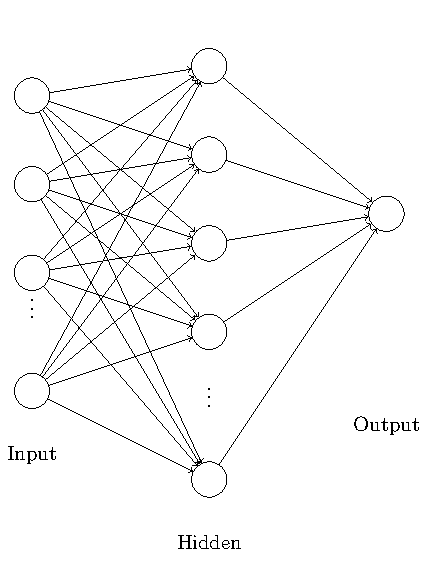
\includegraphics[width=\textwidth]{./project3/tikz/fnn.pdf}
        \caption{FNN}
        \label{subfig:fnn}
    \end{subfigure}
    \hspace{1cm}
    \begin{subfigure}{0.45\textwidth}
        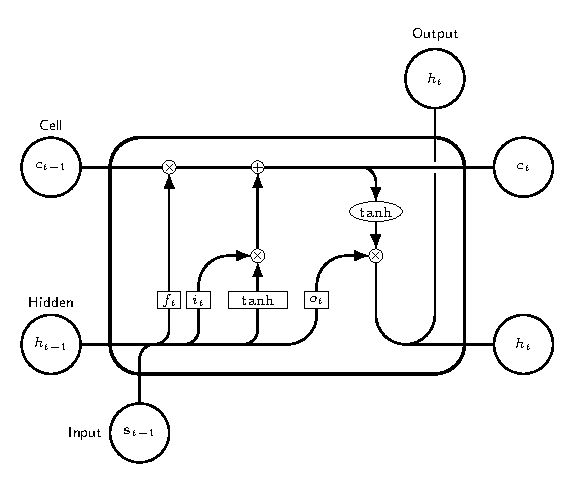
\includegraphics[width=\textwidth]{./project3/tikz/lstm.pdf}
        \caption{LSTM}
        \label{subfig:lstm}
    \end{subfigure}
    \caption{Neural Network Architectures}
    \label{fig:nn}
\end{figure}

Figure~\ref{subfig:fnn} shows a feedforward neural network (FNN) architecture with one hidden layer.
The input layer receives the input features, which are then passed through the hidden layer(s) to the output layer.
Each layer consists of multiple neurons, which apply a non-linear activation function to the weighted sum of the inputs.

\begin{equation}
    f(x; \theta) = f^{(k)}(f^{(k-1)} \cdots (f^{(2)}(f^{(1)}(x;\theta^{(1)});\theta^{(2)} )\cdots ;\theta^{(k-1)});\theta^{(k)}),
\end{equation}

where $\theta = (\theta^{(1)}, \theta^{(2)}, \ldots, \theta^{(k)})$ are the trainable parameters of the neural network, $f^{(i)}$ is the $i$-th layer of the neural network, $x$ is the input feature vector, $f^{(1)}(x;\theta^{(1)}) = x$, $f^{(k)}$ is the output layer, $k$ is the number of layers, and $f^{(i)}$ is the output of the $i$-th layer.
To move from layer $i-1$ to layer $i$,

\begin{equation} \label{eq:neural}
    f^{(i)}(z;\theta^{(i)}) = a^{(i)}(\beta_0^{(i)} + \sum_{j=1}^{p_i} \beta_j^{(i)} z),
\end{equation}

where $a^{(i)}$ are the nonlinear activation functions, $\theta^{(i)} = (\beta_0^{(i)}, \dots, \beta_p^{(i)})$ are the trainable parameters of the $i$-th layer, and $p_i$ is the number of neurons in the previous layer.
Equation~\ref{eq:neural} represents a single neuron in a neural network, which applies a linear transformation to the input followed by a non-linear activation function. 
The linear transformation is similar to the linear regression model in Equation~\ref{eq:regression}, but the non-linear activation function allows the neural network to model complex, non-linear relationships in the data.
The FNN is tuned by adjusting the trainable parameters $\theta$ while fixing the activation functions $a^{(i)}$.
A typical choice for the activation function is the rectified linear unit (ReLU), which is defined as $a(z) = \max(0, z)$.

The key advantage of feedforward neural networks (FNNs) lies in their ability to perform automatic feature engineering without direct human intervention. 
Unlike traditional machine learning models that require manual selection and transformation of input features, neural networks learn to extract and compose features through their hidden layers during the training process. 
Each hidden layer in the network captures higher-level abstractions of the input data by transforming the outputs of the previous layer through nonlinear activation functions~\citep{lecun2015deep}.
Each layer builds upon the representations learned by the previous layer, enabling the network to capture multiple levels of abstraction. This characteristic is crucial for modeling complex datasets with intricate patterns and relationships~\citep{bengio2013representation}.

The last layer of the neural network, known as the output layer, typically performs a linear transformation of the features extracted by the preceding hidden layers. 
With $a^{k}(z) = z$, the last layer is same as a linear regression with its inputs as transformed, high-level features learned by the hidden layers.
By viewing the output layer as performing linear regression on the features learned by the network, we can draw parallels between neural networks and traditional regression models. 
The main difference is that, in neural networks, the input features to the regression model are learned automatically rather than being manually specified.

The most famous theorem in neural network theory is the universal approximation theorem~\citep{hornik1989multilayer}.
It states that given appropriate activation functions $a$, a feedforward neural network with a single hidden layer containing a finite number of neurons can approximate any continuous function on a compact subset of $\mathbb{R}^n$ to arbitrary accuracy. 
Despite this theoretical guarantee for single-layer neural networks, in practice, deep neural networks (DNN) with multiple hidden layers have been shown to be more effective at capturing complex patterns and relationships in data~\citep{lecun2015deep}.
Examples include AlexNet~\citep{krizhevsky2012imagenet}, VGG~\citep{simonyan2014very}, and ResNet~\citep{he2016deep}, which have achieved state-of-the-art performance on image classification tasks.
In this thesis, we focus on the application of deep neural networks, specifically long short-term memory (LSTM) networks, as metamodels for nested simulation procedures in risk management applications.

\subsection{Long Short-Term Memory Networks}

Building upon the capabilities of FNNs, we recognize that while FNNs are successful at capturing complex, nonlinear relationships through automatic feature learning, they are inherently limited when it comes to modeling sequential data or time-dependent patterns. 
This independence assumption limits their effectiveness in modeling financial time series, where temporal dependencies play a critical role. 
The stylized facts of financial time series, such as volatility clustering, fat tails, and autocorrelation, are challenging to capture with traditional feedforward neural networks due to the absence of memory in the model~\citep{cont2001empirical}.

To overcome the limitations of FNNs in handling sequential data, recurrent neural networks (RNNs) were introduced.
In an RNN, the hidden state at each time step is a function of both the current input and the hidden state from the previous time step~\citep{elman1990finding}:

\begin{equation}
    h_t = f(x_t, h_{t-1}; \theta),
\end{equation}

where $h_t$ is the hidden state at time $t$, $x_t$ is the input at time $t$, $h_{t-1}$ is the hidden state at time $t-1$, and $f$ is the recurrent function parameterized by $\theta$.
This architecture enables RNNs to capture temporal dependencies by maintaining a dynamic internal state that reflects the memory of past inputs.
However, traditional RNNs suffer from the vanishing and explodeing gradient problem, which hinders their ability to capture long-term dependencies that often present in financial time series~\citep{bengio1994learning}.
During training, gradients propagated backward through time can either diminish exponentially (vanishing gradients) or grow uncontrollably (exploding gradients).
This limitation is particularly problematic in modeling long-term financial contracts and insurance guarantees, where patterns may span over extended periods.

To address these issues, a long short-term memory (LSTM) network was developed by \citet{hochreiter1997long}.
It is a specialized form of RNNs designed to capture long-term dependencies more effectively with the help of RNN memory cells and gating mechanisms.

\begin{align*}
    i_t &= a(W_i x_t + U_i h_{t-1} + b_i), \\
    f_t &= a(W_f x_t + U_f h_{t-1} + b_f), \\
    o_t &= a(W_o x_t + U_o h_{t-1} + b_o), \\
    g_t &= a(W_g x_t + U_g h_{t-1} + b_g), \\
    c_t &= f_t \odot c_{t-1} + i_t \odot g_t, \\
    h_t &= o_t \odot \tanh(c_t),
\end{align*}

where $i_t, f_t, o_t, g_t, c_t, h_t$ are the input gate, forget gate, output gate, cell input, cell state, and hidden state at time $t$, respectively.
$W_i$, $W_f$, $W_o$, $W_g$, $U_i$, $U_f$, $U_o$, $U_g$ are the weight matrices, and $b_i$, $b_f$, $b_o$, $b_g$ are the bias vectors.
$a$ is the activation function, typically the sigmoid function, and $\odot$ denotes element-wise multiplication.

\begin{equation*}
    a(z) = \frac{1}{1 + e^{-z}}.
\end{equation*}

Figure~\ref{subfig:lstm} shows the architecture of an LSTM network.
The gating mechanisms in LSTMs effectively mitigate the vanishing and exploding gradient problem by regulating the flow of information through the network.
The input gate $i_t$ controls the flow of information into the cell state $c_t$, the forget gate $f_t$ regulates the retention of information in the cell state, and the output gate $o_t$ determines the information passed to the hidden state $h_t$.
The cell input $g_t$ is used to update the cell state based on the input $x_t$ and the previous hidden state $h_{t-1}$.
The cell state $c_t$ acts as a memory unit that stores information over time, while the hidden state $h_t$ captures the relevant information for the current time step.
By incorporating memory cells and gating mechanisms, LSTMs can effectively model long-term dependencies in sequential data in finance and actuarial applications.

This thesis aims to explore the application and noise tolerance of LSTM networks in metamodeling for nested simulation procedures in risk management.
We investigate the performance of LSTM networks in approximating the inner simulation model in a two-stage nested simulation procedure for index-linked insurance contracts.
By leveraging the memory and sequential modeling capabilities of LSTMs, we aim to improve the accuracy and efficiency of nested simulation procedures for risk management applications.

\subsection{Transfer Learning}

% \subsection{Reinforcement Learning}
% Reinforcement learning (RL) is a machine learning technique that learns a policy by interacting with an environment and receiving feedback in the form of rewards.
% In a dynamic heding problem, the policy is a trading strategy that minimizes the risk of the hedged portfolio, the environment contains the financial market dynamics and the contract terms, and the rewards are the negative hedging errors or a risk measure of the hedging portfolio.